\documentclass[tikz,border=10pt]{standalone}
\usepackage{ctex}

\begin{document}
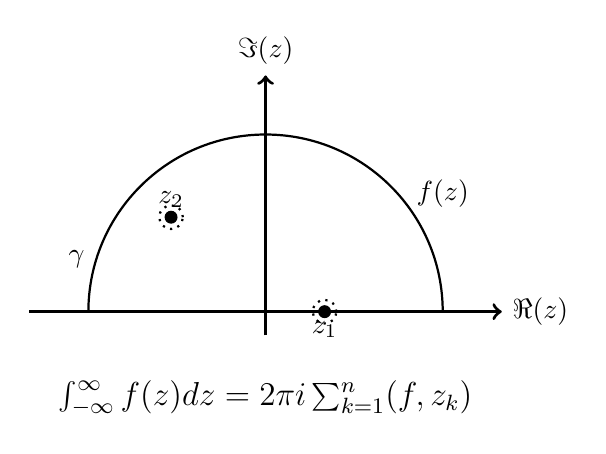
\begin{tikzpicture}[scale=1.5]
  \draw[very thick, ->] (-2,0) -- (2,0) node[right] {$\Re(z)$};
  \draw[very thick, ->] (0,-0.2) -- (0,2) node[above] {$\Im(z)$};
  \draw[black, thick] (-1.5,0) arc (180:0:1.5);
  

  % % Draw the pencil body
  % \filldraw[gray!50, thick] (-2,-0.5) rectangle (2,0.5);
  
  % % Draw the pencil tip
  % \filldraw[black, thick] (2,0.5) -- (4,0) -- (2,-0.5) -- cycle;

  % Inner circles to avoid the singular points
%   \draw[black, thick, dotted] (-0.5,0) arc (180:0:0.5);
%   \draw[black, thick, dotted] (-1.2,0.6) arc (180:0:0.2);
%   \draw[black, thick, dotted] (0.5,0.6) arc (0:180:0.5);
  % Inner circles to avoid the singular points
\draw[black, thick, dotted] (0.5,0) circle (0.1);
\draw[black, thick, dotted] (-0.8,0.8) circle (0.1);
% \draw[black, thick, dotted] (0,-1) circle (0.1);

%   \draw[black, thick, ->] (-1.3,1.3) arc (135:-45:1.8);
  \node[black, below] at (-1.6,0.6) {$\gamma$};
  \node[black, above] at (1.5,0.8) {$f(z)$};
  % \node[black, above] at (0,2.5) {数学物理方法};

%   \node[black, below] at (-1,0.1) {$z_0$};
%   \node[black, above] at (0,2.5) {\LARGE Complex Integration};
%   \node[black, above] at (0,1.8) {\large using the Residue theorem};
%   \node[black, above] at (0,-1) {\large Your Name};
%   \node[black, above] at (0,-1.5) {\large Date};
  \node[black, below] at (0,-0.5) {\large$\int_{-\infty}^{\infty} f(z) dz = 2\pi i\sum_{k=1}^{n} \Res(f, z_k)$};
  
%   \filldraw[black] (-0.5,0) circle (0.05);
%   \node[black, below] at (-0.5,0) {$z_1$};
%   \filldraw[black] (-1.2,0.6) circle (0.05);
%   \node[black, above] at (-1.2,0.6) {$z_2$};
%   \filldraw[black] (0.5,0.6) circle (0.05);
%   \node[black, above] at (0.5,0.6) {$z_3$};

  \filldraw[black] (0.5,0) circle (0.05);
  \node[black, below] at (0.5,0) {$z_1$};
  \filldraw[black] (-0.8,0.8) circle (0.05);
  \node[black, above] at (-0.8,0.8) {$z_2$};
%   \filldraw[black] (0,-1) circle (0.05);
%   \node[black, below] at (0,-1) {$z_3$};

\end{tikzpicture}
\end{document}
